%! Author = marcusdesai
%! Date = 16/08/2023

% Preamble
\documentclass[border=5pt]{standalone}

% Packages
\usepackage{amsmath}
\usepackage{tikz}
\usetikzlibrary{automata, positioning, arrows}

% Document
\begin{document}

    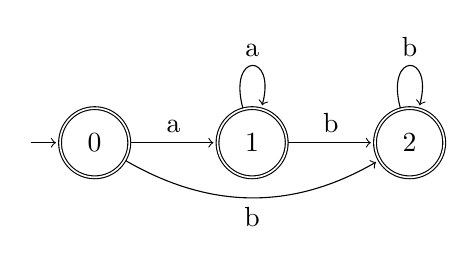
\begin{tikzpicture}[shorten >=1pt, node distance=2cm, on grid, auto]
        \tikzset{initial text={},initial where=left}
        \tikzstyle{every initial by arrow}=[initial distance=1em,inner sep=0pt]

        \node[state,initial,accepting] (q_0) {$0$};
        \node[state,accepting] (q_1) [right=of q_0] {$1$};
        \node[state,accepting] (q_2) [right=of q_1] {$2$};
        \path[->]
        (q_0) edge node {a} (q_1)
        (q_0) edge [bend right] node[below] {b} (q_2)
        (q_1) edge [loop above] node {a} (q_1)
        (q_1) edge node {b} (q_2)
        (q_2) edge [loop above] node {b} (q_2);
    \end{tikzpicture}

\end{document}
